\subsection{Historical Classical Evidence: Array Size and Useful Structure}
\begin{figure*}[!t]
\centering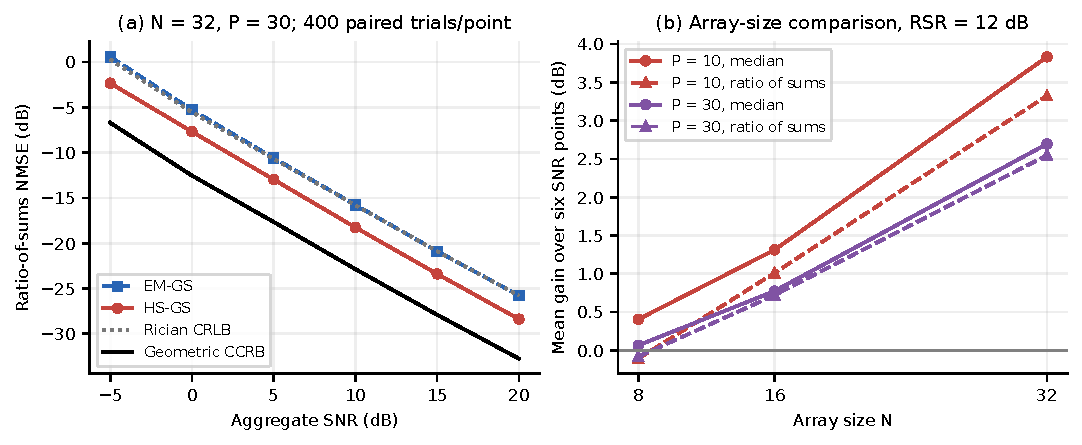
\includegraphics[width=\textwidth]{classical_array.pdf}
\caption{Classical study. Left: NMSE and information references at $N=32$, $P=30$, RSR 12~dB. Right: HS-amplitude gain versus array size for two pilot counts. HS-GS denotes four-sweep HS-amplitude. Solid gain curves average paired medians over six SNRs; dashed curves average ratio-of-sums gains.}
\label{fig:classical}
\end{figure*}
At $N=32$, $P=30$, RSR 12~dB, HS-amplitude gains 2.54--2.97~dB in paired median over EM-GS across six SNRs, averaging 2.70~dB (Fig.~\ref{fig:classical}). Ratio-of-sums gaps are 2.38--2.90~dB. At SNR at least 5~dB, EM-GS is within 0.108~dB of the Rician CRLB. The geometric CCRB is 6.95--7.06~dB below that reference, while HS-amplitude remains 4.37--4.85~dB above it. These local unbiasedness references do not establish efficiency or attainable headroom for the biased filtered estimates.

Averaging two pilot counts and six SNRs, paired-median gains are 0.236, 1.044 and 3.264~dB for $N=8,16,32$; ratio-of-sums gains are $-0.095$, 0.866 and 2.938~dB. Larger arrays provide more spatial samples of the same paths. At $N=8$, maximum Hankel rank is four and filtering is bypassed in 42.94\% of trials. A positive median alongside a negative total-error gain shows why aggregation matters.

\subsection{Effective Rank and Filtering Bias}
For the true noiseless Hankel spectrum, define effective rank~\cite{royvetterli2007}
\begin{equation}
 r_{\rm eff}=\exp(-\textstyle\sum_i p_i\log p_i),\qquad \rho=r_{\rm eff}/q.
\end{equation}
A spectrum dominated by a few values has low effective rank even if its algebraic rank is larger. We report median $\rho$ over users and worlds. This true-channel diagnostic is not available to the estimator.
\begin{figure}[!t]
\centering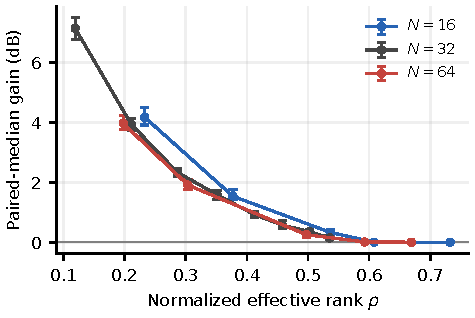
\includegraphics[width=\columnwidth]{effective_rank.pdf}
\caption{Four-sweep HS-amplitude paired-median gain versus true-channel normalized effective rank. Arrays use $P=20$, RSR 10~dB and the same random-SNR distribution. Bars are pointwise paired-bootstrap intervals. This is a diagnostic trend, not an observable switching threshold.}
\label{fig:rank}
\end{figure}
Across the matched array tests, hard-rank benefit generally falls as $\rho$ rises (Fig.~\ref{fig:rank}). At $N=32$, $\rho=0.536$ gives median gain 0.141~dB with interval $[0.090,0.211]$~dB. A value near one-half of capacity marks a small benefit here, not a universal threshold. At $N=16$, $L=14$, $\rho=0.732$, forcing rank seven loses 0.154~dB, with interval $[0.111,0.201]$~dB for the loss.

Adaptive rank does not protect every channel: at $N=32$, $L=14$, SNR 0~dB, HS-amplitude is worse than EM-GS in 47.75\% of 400 worlds. Selecting below the physical path count is not always harmful either. At $L=7$, SNR 0~dB, 78.75\% select below rank seven, but only 8.75\% of all worlds are worse than EM-GS.

Classical smooth filtering gains 0.914, 1.382 and 1.413~dB over four hard sweeps at SNR 0~dB for $L=3,7,14$. At 10~dB, gains are 0.005, 0.623 and 0.773~dB; the first interval includes zero. Learning is therefore not required to improve hard truncation. A separate historical check also finds one hard sweep better than four in all six cells by 0.275--0.652~dB. More filtering is not automatically better.

